\chapter{Senzory}

Senzory k~projektu Pletačka IoT jsou postavené na mikročipu ESP32 a~modulech TTGO~T-Display.
Celý tento systém je navržen tak, že na každém pletacím stroji je jeden senzor.
Každý z~těchto senzorů má svoje jedinečné číslo, pod kterým posílá naměřená data na server.
Senzor je napájen z~5 nebo 24 voltů a~má spotřebu 120 mA.
Návrh senzorů i~jejich software mám verzovaný nástrojem Git ve veřejném repozitáři~na GitHubu.\newline
GitHub: \href{https://github.com/Pletacka-IoT/Pletacka-board}{Pletacka-board}\cite{PL_BOARD}

\section{Procesor}
Jako řídící procesor jsem zvolil čip ESP32, protože je velice výkonný a disponuje konektivitou WiFi.
Procesor obsahuje 4MB flash paměti sloužící k ukládání programu.

Po prozkoumání trhu jsem našel modul TTGO~T-Display, který kombinuje barevný displej s čipem ESP32.
Tato kombinace mi vyšla jako nejlepší, spojuje totiž bezproblémovou komunikaci s tímto displejem a zároveň jednoduchou výměnu při nefunkčnosti čipu.


\section{Vstupy a výstupy}
Napájecí okruh pletacího stroje pracuje s napětím 24 voltů, proto jsem potřeboval, aby i moje elektronika, dokázala takovéto napětí zpracovávat.

Jeden vstup je připojen ke světlu které signalizuje zastavení stroje a druhý k senzory, který zaznamenává dopletenou ponožku.
Tyto vstupní signály jsou připojeny na optočleny, které vodivě oddělí vstupní napájení a na výstupu máme pouze třívoltový signál, který je zpracovatelný čipem.



\section{Vlastní PCB}

K vytvoření vlastní desky mě vedlo několik faktorů. První z nich byla velikost celé elektroniky. 
Nevýhodou elektroniky postavené z existujících modulů je právě jejich velikost, moduly se dají jednoduše skládat k sobě ale zabírají spoustu místa. 
 
Dalším důvodem je replikovatelnost. Těmito deskami plánuji osadit celou firmu, díky čemuž bylo zapotřebí vyrobit 3O stejných elektronických desek.

Desky jsem si tedy nechával vyrábět v čínské firmě JLCPCB. Jejich výroba je velmi precizní a dokáží desku i osadit vybranými součástkami.



\section{1. verze - univerzální sensorika}

První verzi jsem pojal jako testovací. Bylo tedy třeba navrhnout univerzální desku a~otestovat celý systém.\newline

Při~navrhování senzoru jsem si stanovil tyto body:
\begin{itemize}
    \item ESP32 s~barevným displejem
    \item vstup ze 4 periferií
    \item vstupní napětí od 10 do 25V
    \item teplotní čidlo
    \item tři~barevné diody
    \item čtyři~uživatelská tlačítka
\end{itemize}

% \subsection{Elektronika}
% % Modul TTGO~T-Display jsem zvolil kvůli jeho jednoduché práci s displejem. 
% Modul TTGO~T-Display jsem zvolil z toho důvodu, že má přímo v sobě integrovaný mikročip ESP32.
% Ten je dostatečně výkonný a disponuje konektivitu Bluetooth a WiFi. 

\subsection{Řídící deska}
Návrh desky jsem tvořil v~aplikaci EAGLE od společnosti Autodesk. 
Deska má rozměry 75 na 60 mm a~v~každém rohu má upevňovací otvory.
Kabely se do desky připojují pomocí 5 mm svorkovnice.
Na vstupu napájení je měnič napětí, který pracuje v~rozsahu od 10 do 25 voltů a~na výstupu dává 5V. 

Řídící procesor celé desky je modul ESP32 TTGO T-Display.
Tento čip také zajišťuje WiFi konektivitu s~okolím a~odesílá naměřená data na server.
Pro univerzální detekování vstupů z~periferií se využívají optočleny, které předávají signál do mikroprocesoru.
K~uživatelskému ovládání senzoru jsou zde čtyři~programovatelná tlačítka a~tři~indikační diody.
Aktuální naměřená data se zobrazují na displeji a~informují obsluhu o~zastavení stroje a~počtu upletených párů.
Senzor je také schopen zaznamenávat data ze čtyř vstupů a~teplotu z~teplotního senzoru. Viz obrázek \ref{fig:SenzorV1}.

\subsection{Uchycení}
Krut řídící desky je vytisknutý na 3D tiskárně z~materiálu PETG.
Na přední straně je průhled z~plexiskla na barevný displej a~okolo něj jsou rozmístěná uživatelská tlačítka.
Na boční straně krytu jsou připravené dvě drážky na protažení stahovacích zip pásků pro uchycení na sloupek stroje.
Signálové kabely jsou poté svedeny po konstrukci stroje až k~periferiím.


\subsection{Program}
K~programování využívám aplikaci Visual Studio Code s~rozšířením PlatformIO, která je navržena k~programování mikrokontrolérů. 
Zdrojový kód mám napsaný v~jazyce C++.
Program se skládá z~několika vláken, které se pravidelně spouštějí a~vykonávají.
První a~zároveň nejdůležitější vlákno je senzorové.
Zde se periodicky kontroluje stav periferií a~při~změně se odešle událost na server.
Další vlákno zajišťuje pravidelné vykreslování dat na displej a~zbylá vlákna se starají o~správný chod senzoru.
Software také obsahuje ladící mód, ve kterém si administrátor může zobrazit stav senzoru v~mobilní aplikaci a~jednodušeji tak hledat potenciální chybu. 


\begin{figure}[htbp]
    \centering
    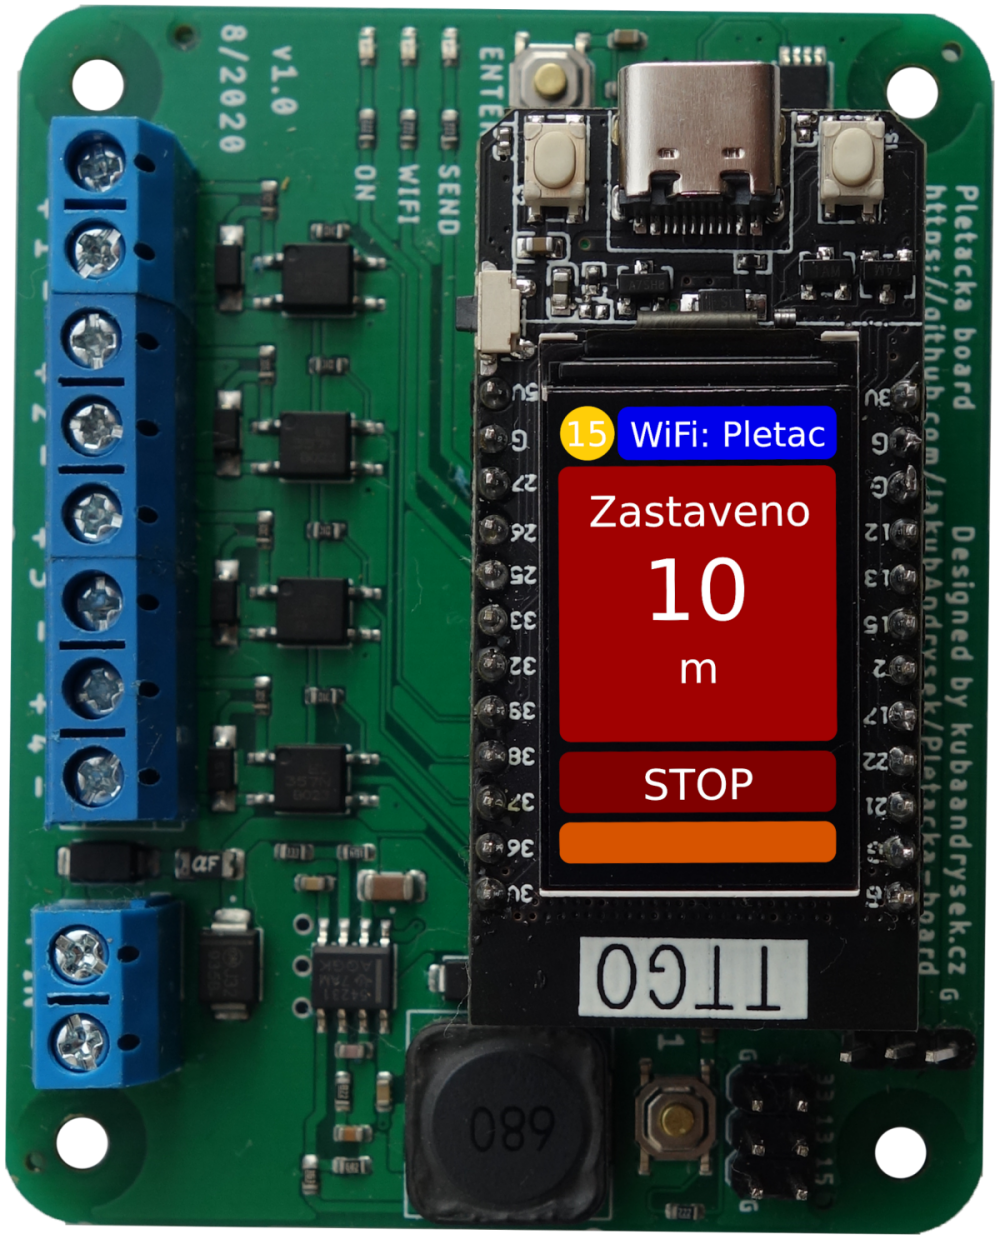
\includegraphics[width=\textwidth/2]{img/V1-deska-esp-screen.png}
    \caption{Senzor - 1. verze}
    \label{fig:SenzorV1}
\end{figure}


\newpage





% 2. verze - speciální senzorika
\section{2. verze - speciální senzorika}

Po měsíci testování jsem zhodnotil využití jednotlivých součástek a~následně jsem vytvořil nový seznam požadavků, přizpůsobený pro lepší chod senzoru.
Zařízení je díky tomu mnohem menší, levnější a~softwarově rychlejší.

\begin{itemize}
    \item vstup pouze ze 2 periferií
    \item vstupní napětí již od 5V
    \item zredukování rozměrů
    \item moderní USB-C konektor
    \item zredukování na dvě tlačítka a~dvě indikační diody
    \item možnost přímého napájení senzoru bez měniče
\end{itemize}

\subsection{Řídící deska}
Návrh druhé desky jsem se rozhodl udělat v~open source aplikaci KiCad.
Z uživatelského hlediska se sní pracuje o něco rychleji díky jednoduchým klávesovým zkratkám. 
Dalším důvodem pro zvolení této aplikace bylo rozšíření KiKit, která razantně zjednodušuje export výrobních podkladů.
Zatímco v dříve používané aplikaci Eagle jsem při každé změně musel projít zdlouhavým procesem exportu, nyní v linuxovém terminálu stačí zavolat `make' a celý proces se vykoná automatizovaně bez nutnosti editace dat.

Rozšíření KiKit jsem také začal používat k automatizovanému generování dokumentace k plošným spojům.
Rozvržení webové stránky si uživatel nastaví v konfiguračním souboru a následně při každé změně se stránka přegeneruje a aktualizuje.

V~novém návrhu jsem se~především zaměřoval na~rozměr desky, ten aktuálně činí 32$\times$76 mm, což je o~46 procent menší plocha než u~první verze.

Deska si~zachovala stejný procesor ESP32 s~displejem, ale přišla~o~dvě~tlačítka a~jednu indikační diodu.
V~senzoru~se také změnilo zapojení měniče napětí.
Nově dokáže pracovat již od~5V, které následně mění na~3,3V.
Na~bočních stranách desky vznikla také nová "křidélka" pro zasunutí~do vylepšeného krytu.



\subsection{Uchycení}
Druhá verze využívá stejného principu uchycení, jako ta~předchozí. 
Mění se~zde však spojení krabičky se~senzorovou deskou. 
V~nové verzi jsem desku navrhl tak, aby se~dala jednoduše zasunout~do kolejnic které jsou předtištěné v~krabičce a~následně zafixovat šroubkem ze~zadní strany.
To~umožňuje jednoduchou montáž~a~rychlé připojení.
Tento návrh už~má~také vyřešené zafixování kabelů ke~konstrukci krabičky pomocí 3D tištěných svěrek.


\subsection{Program}
Program druhé verze vychází z~minulé, ale přináší s~sebou nové funkce a~vylepšuje stávající.
Novou funkcionalitou je například automatická aktualizace programu přes WiFi, kterou nadále zdokonaluji.
Další vylepšení jsem provedl u displeje, který dokáže zobrazit více údajů a~automaticky mezi nimi přepínat.

\begin{figure}[htbp]
    \centering
    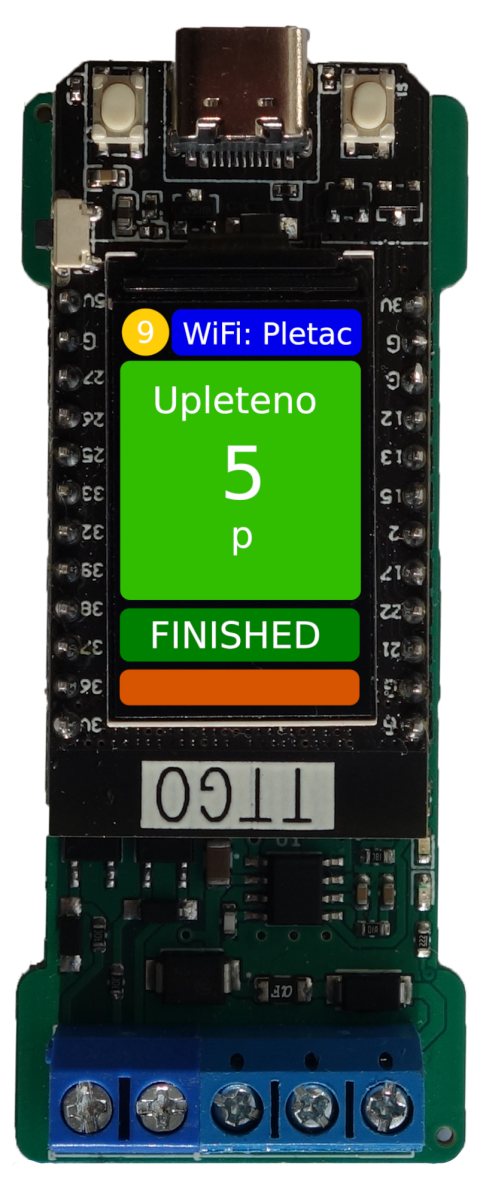
\includegraphics[width=\textwidth/3]{img/V2-deska-esp-screen.png}
    \caption{Senzor - 2. verze}
    \label{fig:SenzorV2}
\end{figure}


\newpage